% $Id$
% Author:	Daniel Bosk <daniel.bosk@miun.se>
\documentclass[a4paper]{article}
\usepackage[utf8]{inputenc}
\usepackage[T1]{fontenc}
\usepackage[english,swedish]{babel}
\usepackage{natbib}
\usepackage{prettyref}
\usepackage{varioref}
\usepackage[binary]{SIunits}
\usepackage{graphicx}
\bibliographystyle{sweplnat}

\author{Daniel Bosk}
\title{Testdokument}
\date{\today}

\begin{document}
	\maketitle

	\begin{abstract}
    En första paragraf kan se ut så här.
		Det krävs en del text för att det ska se vettigt ut.
		Det räcker inte med några få ord för då fyllar man inte ens ut en rad.

		Det där borde räcka för en paragraf, eller stycke.
		Detta är en ny paragraf.

		Eftersom att detta dokument använder dokumentklassen article finns inga 
		kapitel.
		Därför diskuterar vi nästa del i ett avsnitt.
	\end{abstract}

	\tableofcontents

	\section[Första avsnittet]{Det första avsnittet i dokumentet}
	\label{sec:First}
  Här fyller vi på med några meningar för att fylla ut en paragraf och sedan 
  skapa ytterligare en.

	Här kommer nästa, en mycket kort paragraf.

	\subsection[Delavsnittet]{Ett lämpligt delavsnitt}
	\label{sub:Del}
  Här fyller vi på med några meningar för att fylla ut en paragraf och sedan 
  skapa ytterligare en.

	Här kommer nästa, en mycket kort paragraf.


	\section{Referenshantering}
	\label{sec:Ref}
  Enligt \citet{Knuth1997tao} finns ingen algoritm för att lösa problemet.

	Vi har summan \( \sum_{i=1}^n i = \frac{n (n + 1)}{2} \).
  Men sedan har vi även summan \[ \sum_{i=1}^n i = \frac{n (n + 1)}{2}. \]
	Detta ger resultatet:
	\[ f(a) = \left\{
		\begin{array}{ll}
			y & \text{om } a=x \\
			x & \text{om } a=y
		\end{array}
		\right\} = f^{-1}(a). \]


	\section{Figurer och tabeller}
	\label{sec:FigTab}
  För att illustrera detta se \prettyref{fig:bild} och 
  \prettyref{tbl:SannolikhetstabellSpråk}.
	Men först bör du ha läst \prettyref{sec:First}.

	\begin{figure}
		\centering
		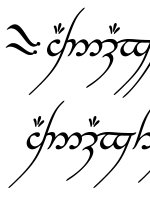
\includegraphics[width=0.2\linewidth]{tengwar.jpg}
		\caption{En bild föreställande J. R. R. Tolkiens tengwar.}
		\label{fig:bild}
	\end{figure}
	\begin{table}
		\centering
		\begin{tabular}{r|cccccccccc}
			\hline\hline
			\(\alpha\) & a & b & c & d & e & f & g & h & i & j \\
			\(P_E(\alpha)\) & 8.2  & 1.5 & 2.8 & 4.3 & 12.7 & 2.2 & 2.0 & 6.1 & 7.0 & 0.2 \\
			\(P_S(\alpha)\) & 9.3  & 1.3 & 1.3 & 4.5 & 9.9 & 2.0 & 3.3 & 2.1 & 5.1 & 0.7 \\
			\hline\hline
		\end{tabular}
		\caption{Tabell av sannolikhetsfunktionen för bokstäver i det engelska och det svenska språket, \(P_E\) respektive \(P_S\), angiven i procent med en decimals noggrannhet.}
		\label{tbl:SannolikhetstabellSpråk}
	\end{table}

	Därefter kan du beräkna hur många \mega\byte{} det krävs för en \giga\byte.
	Hur skiljer sig en \gibi\byte{} jämfört med en \giga\byte?
	Vilken hastighet, angiven i \giga\bit\per\second, motsvarar 
	\unit{10}{\gibi\bit\per\second}.
	Är det nödvändigt att ha en hastighet på \unit{10}{\tera\bit\per\second}?


	\bibliography{literature}
\end{document}
